\chapter{Revisão de Literatura}

% \section{Planejamento e estimativas em metodologias ágeis}

  As metodologias ágeis se baseiam nos valores ágeis publicados no Manifesto Ágil
  (BECK, 2001 \textit{apud} \citeonline{cohn06}), que são:

  \begin{itemize}
   \item Indivíduos e interações entre eles mais que processos e ferramentas;
   \item Software em funcionamento mais que documentação abrangente;
   \item Colaboração com o cliente mais que negociação de contratos;
   \item Responder a mudanças mais que seguir um plano.
  \end{itemize}

 Seguir uma metodologia ágil em um projeto, também implica em uma abordagem ágil nas estimativas e planejamento, seguindo
 os valores supracitados \cite{cohn06}. Conceitos importantes são necessários para entender o planejamento e estimativas
 num projeto ágil, como: iteração e \textit{sprints}, \textit{story points}, \textit{velocity}, entre outros.
 Esses conceitos serão devidamente aprofundados nas próximas seções.

\section{Tempo de trabalho: \textit{Sprints}}

 Times ágeis trabalham em iterações, que são um período de tempo fixo (\textit{time-boxed}) curto, de não mais que
 um mês de duração \cite{cohn06} \cite{scrum13}. O \textit{Scrum}, um \textit{framework} estrutural ágil,
 traz o conceito de \textit{Sprint} para o processo de desenvolvimento, que nada mais é que um \textit{container}
 temporal fixo para outros eventos do \textit{Scrum} \cite{scrum13}. Numa \textit{Sprint} é produzido um incremento
 do \textit{software}, com base no que foi estabelecido como escopo daquela \textit{Sprint}. Como uma \textit{Sprint} possui
 a duração fixa, mesmo que uma funcionalidade não tenha sido completada nesta \textit{Sprint}, a mesma é encerrada no prazo
 que foi determinado \cite{cohn06}.

 De acordo com \citeonline{scrum13}, a
 \textit{sprint} é composta pela reunião de planejamento da \textit{sprint}, reuniões diárias, trabalho de desenvolvimento,
 revisão da \textit{sprint} e retrospectiva da \textit{sprint}. Os esforços de estimativas se concentram na reunião de
 planejamento da \textit{sprint}, onde são estimadas as histórias de usuários. No começo de cada \textit{sprint}, o time
 incorpora todo o conhecimento obtido com a \textit{sprint} passada para adaptar e ajustar o planejamento da próxima
 \textit{sprint} \cite{cohn06}.

\section{Estimativas com \textit{Story Points}}

 Em um projeto ágil
 que utiliza histórias de usuário, pode-se estimar o tamanho de uma história em \textit{story points}.
 \textit{Story points} representam o tamanho geral de uma história, envolvendo o esforço necessário, a complexidade e os
 riscos inerentes para desenvolver a história \cite{cohn06}. O número atribuído à história como seu tamanho não é relevante,
 o que importa é o valor relativo entre as histórias, que é obtido por comparação entre elas \cite{cohn06}.

  \subsection{\textit{Velocity}}

    Numa abordagem ágil, a estimativa do tamanho é separada da estimativa da duração \cite{cohn06}.
    Com o tamanho estimado, é preciso de outro conceito para se calcular a duração, o \textit{velocity}.
    O \textit{velocity} mede a taxa de progresso do time, dizendo quantos pontos o time é capaz de desenvolver
    numa \textit{sprint}, podendo ser calculado como a soma dos pontos concluídos durante a iteração \cite{cohn06}.
    A melhor forma de se estabelecer o \textit{velocity} para um time é executando uma ou duas iterações e estimar o
    \textit{velocity} a partir do \textit{velocity} observado \cite{cohn06}.

  \subsection{Estimando a duração}

    Com o tamanho do \textit{software} e o \textit{velocity} do time de desenvolvimento conhecido, fica fácil estimar
    um prazo para o projeto, dividindo o tamanho pelo \textit{velocity}, obtendo assim a quantidade de \textit{sprints}
    necessárias, e multiplicando pelo tamanho da \textit{sprint} \cite{cohn06}.

    Utilizando uma abordagem por \textit{story points} em um projeto, separa-se completamente a estimativa do esforço
    necessário da estimativa da duração do projeto, permitindo que ambos sejam estimados independentemente. A estimativa de
    duração do projeto passa a ser derivada da estimativa de esforço \cite{cohn06}.

  \subsection{Escala das estimativas}
  \label{estimation_scales}

      Utilizar uma única ordem de magnitude gera estimativas melhores (Miranda 2001; Saaty 1996 \textit{apud} \cite{cohn06}).
      De acordo com \citeonline{cohn06}, uma escala de estimativa bastante utilizada e que se mostra bastante eficaz é a
      sequência \textit{Fibonnaci}, que consiste em pontuar as histórias utilizando algum número da
      sequência 1, 2, 3, 5, 8, 13, [...]. É importante estabelecer um valor máximo para a sequência para manter o intervalo
      conhecido e não demasiado grande.

  \subsection{\textit{Planning Poker}}

    O \textit{Planning Poker} é uma técnica utilizada para estimativas ágeis que envolve as três técnicas de estimativa
    mais comuns (opinião do especialista, analogia e desagregação), gerando estimativas rápidas e confiáveis \cite{cohn06}.

    Todos os desenvolvedores participam do \textit{Planning Poker}, que se inicia com a entrega das cartas que contém os
    valores válidos para as histórias na escala definida (vide a sub-seção \ref{estimation_scales}).
    Uma história é selecionada e é lida sua descrição pelo moderador
    do jogo (usualmente o \textit{Product Owner}, que não participa das estimativas) para que então os jogadores possam
    avaliar a história e pontuá-la. Se houver divergências entre as pontuações, é iniciado um debate para que seja definida
    a pontuação final da história. Uma nova rodada é jogada para a mesma história caso os participantes não
    entrem em um consenso \cite{grenning02}.

    O objetivo é fazer com o que os participantes convirjam para uma estimativa que será utilizada como pontuação da
    história, lembrando que a proposta do \textit{Planning Poker} não é gerar uma estimativa acurada que perdure por
    todo o ciclo de desenvolvimento, pois para atingir tal estimativa seria gasto um esforço
    desnecessário \cite{cohn06} \cite{grenning02}.

    \citeonline{cohn06} diz que existe uma acurácia máxima para uma estimativa
    em relação ao esforço necessário para realizá-la, como ilustra a Figura \ref{fig:effort_accuracy}.
    Portanto, não é preciso um debate demorado e detalhado durante o \textit{Planning Poker} para se definir
    o tamanho das histórias, objetivando sempre ficar do lado esquerdo da curva apresentada na Figura \ref{fig:effort_accuracy}.



    \begin{figure}[!htb]
      \centering
      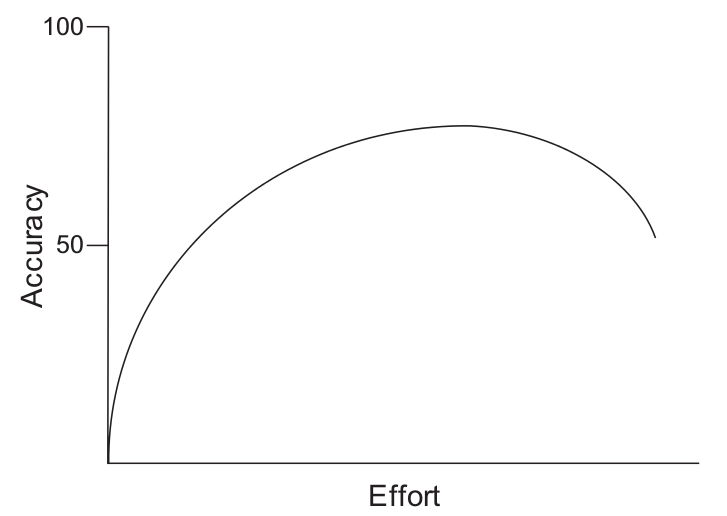
\includegraphics[scale=0.4]{figuras/effort_accuracy}
      \caption[Relação entre a acurácia e o esforço realizado para a estimativa.]
	      {Relação entre a acurácia e o esforço realizado para a estimativa. Fonte: \cite{cohn06}}
      \label{fig:effort_accuracy}
    \end{figure}

  \section{\textit{Burndown}}

    Objetivando conhecer a velocidade com a qual a equipe realiza seu trabalho, elabora-se um gráfico \textit{burndown} o qual é responsável por mostrar a quantidade de trabalho restante no início de cada iteração. Além disso, essa ferramenta se torna um poderoso indicador visual da rapidez com que uma equipe está se movendo em direção a sua meta \cite{cohn06}. O \textit{burndown} pode ser calculado por \textit{sprint}, por \textit{release}, por um projeto como um todo. No âmbito deste trabalho foi trabalhada a ideia de realização de \textit{burndown} por \textit{sprint}.

    Em um gráfico \textit{burndown} por \textit{sprint} apresenta-se no eixo vertival o número de pontos de história restantes na sprint e no eixo horizontal os dias ao longo da \textit{sprint} \cite{cohn06}.
    
  \section{Administração e Governança da Tecnologia da Informação (TI)}

    A área ou função organizacional formal de uma empresa responsável pela prestação de serviços tecnológicos dentro da mesma é denominada departamento ou área de TI. Sua principal função é a de manter os equipamentos (hardware), sistemas e programas (software), armazenagem de dados e redes de comunicação. É composta principalmente de especialistas tais como programadores, analistas de sistemas, líderes de projetos e gerentes de sistemas de informações (J. Laudon \& K. Laudon, 2004).

    Para endereçar uma série de problemas na administração da área de TI, vem sendo adotada por grande parte das organizações, a governança de TI. Seu principal objetivo é o de melhorar a comunicação entre a área de TI e o  negócio assim como aumentar a consistência e a transparência de seus processos internos e de sua gestão em si (Laurindo, 2008).

    Nas últimas três décadas, além do aumento da complexidade das aplicações de TI, houve também o aumento da preocupação de gestores de melhorar a administração dessa área de TI (Laurindo, 2008).

    Isso ocorre pelo fato de qualquer empresa líder ter acesso a semelhantes recursos ou capacidades de TI. Dessa forma, o que determina então a vantagem ou desvantagem competitiva de uma empresa é a diferença na forma como sua TI é administrada (Keen, 1993).

    A primeira medida para formular a governança de TI é determinar quem (um dono responsável) deve tomar cada tipo de decisão e que seja responsabilizado por seus resultados. Dessa forma, a governança de TI consiste em um quadro de referência que contempla responsáveis pelas decisões (ou donos das decisões) e responsabilidades e práticas para estimular comportamentos desejáveis no uso da TI (Weill \& Ross, 2005).

    Portanto, governança contribui para um melhor alinhamento entre a TI e o negócio. Porém, além disso as empresas necessitam de um processo que as ajude a realizar um planejamento estratégico da TI de maneira eficaz. Este planejamento é um conjunto de objetivos futuros que descreve o alicerce da TI e os principais projetos de Sistema de Informação (SI) necessários para alcançar as metas da organização (Turban, Rainer \& Potter, 2005).

    Laudon, J. P. \& Laudon, K. C. (2004). Sistemas de informação gerenciais: administrando a empresa digital (5a ed.). São Paulo: Prentice Hall.

    Laurindo, F. J. B. (2008). Tecnologia da informação: planejamento e gestão de estratégias. São Paulo: Atlas.

    Keen, P. G. W. (1993). Information technology and the management difference: a fusion map. IBM Systems Journal, 32(1), 17-39.

    Weill, P. \& Ross, J. (2005). A matrixed approach to designing IT governance. MIT Sloan Management Review, 46(2), 26-34.

    Turban, E., Rainer, R. K. \& Potter, R. E. (2005). Administração de tecnologia da informação: teoria e prática (3a ed.). Rio de Janeiro: Elsevier.

  \section{Projetos de TI}

    Dentre as definições de um projeto a mais comum e aceita é aquela que o define como um esforço temporário empreendido para criar um serviço, produto ou resultado exclusivo. Por ser temporário, possui sempre uma data de início e fim definidas. Atingi-se o fim quando os objetivos iniciais do projeto tiverem sido alcançados. Embora elementos repetitivos possam estar presentes dentro de projetos distintos, essa repetição não muda a característica fundamental de cada projeto: a natureza exclusiva de cada um desses empreendimentos (Project Management Institute [PMI], 2008).

    Algo que deve ser levado em conta é que muitos dos projetos de TI são complexos em termos de inovação tecnológica e/ou número de interfaces entre os atores (stakeholders) envolvidos. Isso proporciona a esses projetos um alto nível de incerteza relacionado com a tecnologia envolvida, com a data de entrega e com o horizonte de stakeholders envolvidos (Vaagaasar, 2011).

    Assim como todo projeto, mas em especial, os projetos de TI por apresentarem essas particularidades, incorrem em falhas que – se não gerenciadas da maneira correta levam a desperdícios, atrasos, entre outros problemas. Além, é claro, de ter uma influencia negativa na estratégia da organização e outras consequências muitas vezes desastrosas (REFERÊNCIA - OMAR).

    Chapters Brasileiros do PMI. (2008). Estudo de benchmarking em gerenciamento de projetos Brasil 2008. Recuperado em 18 de novembro de 2015, de http://www.pmsurvey.org.

    Vaagaasar, A. L. (2011). Development of relationships and relationship competencies in complex project. ISMPB, 4(2), 294-307.


  \section{Atraso}

    Mesmo com todo o planejamento e medidas tomadas no mundo de desenvolvimento de software pode ocorrer atrasos em entregas. Para este trabalho cpmsideramos como atraso o fato de não finalizar todas as tarefas que haviam sido propostas para a entrega.


%Ideias para possíveis tópicos
% \section{Metodologia ágil}
% % 	\subsection{Estimativas em \textit{StoryPoints}}
% 	\subsection{Velocity}
% 	\subsection{Prazo de entrega
% 	\subsection{Atrasos na entrega}



